\begin{graphicspathcontext}{{./chapters/simulation/imgs/},{./chapters/simulation/imgs/auto/},{./chapters/mas/imgs/auto/}\old}

\begin{frame}{What is the Agent Environment?} 
	\begin{definitionblock}{Agent Environment \cite{weyns2007environment}}
		The environment is a first-class abstraction that provides the agents with a computational infrastructure and a set of services to facilitate agent interaction and situatedness.
	\end{definitionblock}
	
	\begin{block}{Properties}
		\begin{description}
		\item[Situatedness] Agents are situated in the environment; they perceive it through sensors and act upon it through actuators
		\item[Medium for interaction] The environment mediates all interactions among agents (indirect, e.g., stigmergy)
		\item[Active role] The environment is not merely a passive container; it has its own dynamics, laws, and computational processes independent of agents
		\item[Services provider] The environment offers services to agents (e.g., communication, coordination, spatial reasoning)
		\end{description}
	\end{block}
\end{frame}

\begin{frame}{{Formal Definition} of the Agent Environment} 
	\[E = \langle O, Ag, R, L, \Omega, \tau \rangle\]
	\begin{stabularx}{l|X}
		\tabularhead{Symbol}{Description} \\
		$O$ & Set of objects (passive entities) in the environment \\
		$Ag$ & Set of agents situated in the environment \\
		$R$ & Set of relations among objects and agents \\
		$L$ & Set of laws governing the environment's dynamics \\
		$\Omega$ & Set of observable properties of the environment \\
		$\tau$ & The time model governing state transitions \\
	\end{stabularx}
\end{frame}

\sidenote{Mix of the archectures given by \cite{weyns2007environment,Weyns05,Viroli07}}
%\animatedfigureslide[width=.75\linewidth]{Environment Layers}{environment_layers} 
\figureslide{Environment Layers}{environment_layers_full} 

\begin{frame}{{Key Properties} of the Agent Environment}
	\vspace{-.25cm}
	\begin{columns}
		\begin{column}{.2\linewidth}
			\begin{bottomarrowsequence}
				\only<1>{\arrow[bg=CIADgreen]{Observability}}
				\only<2->{\arrow{Observability}}
				\only<2>{\arrow[bg=CIADgreen]{Determinism}}
				\only<1,3->{\arrow{Determinism}}
				\only<3>{\arrow[bg=CIADgreen]{Dimensionality}}
				\only<1-2,4>{\arrow{Dimensionality}}
				\only<4>{\arrow[bg=CIADgreen]{Dynamicity}}
				\only<1-3>{\arrow{Dynamicity}}
			\end{bottomarrowsequence}
		\end{column}
		\begin{column}{.8\linewidth}
			\only<1>{
				\smaller
				\begin{block}{Fully Observable Environment}
					\begin{itemize}
					\item \Emph{All aspects} of the environment are visible
					\item \Emph{Complete, accurate, and up-to-date} knowledge of the environment state
					\end{itemize}
				\end{block}
				\begin{block}{Partially Observable Environment}
					\begin{itemize}
					\item Observability is limited in space and time and specific to each agent
					\item Agent maintains \Emph{internal model} to track sensed information
					\item \Emph{Other agents' intentions} are not observable, even if their actions are
					\end{itemize}
				\end{block}
				\centering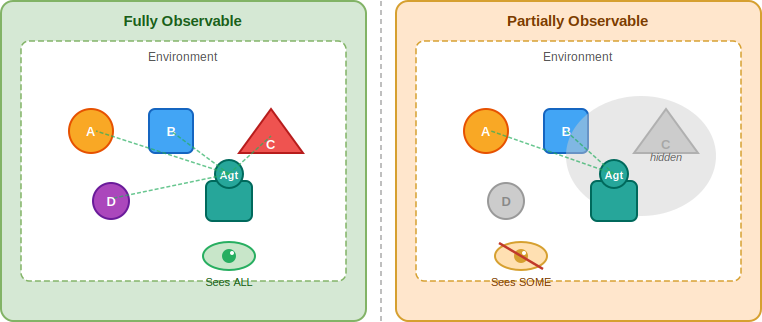
\includegraphics[width=.6\linewidth]{environment_observability}
			}
			\only<2>{
				\smaller
				\begin{columns}
					\begin{column}{.5\linewidth}
						\begin{block}{Deterministic Environment}
							\Emph{Next state} of the environment is \Emph{completely predictable} from the current state and the action executed by the agent
						\end{block}
					\end{column}
					\begin{column}{.5\linewidth}
						\begin{block}{Stochastic Environment}
							\Emph{Next state} has \Emph{some uncertainty} due to randomness, incomplete or inaccurate models, incomplete sensor coverage
						\end{block}
					\end{column}
				\end{columns}
				\vspace{-.2cm}
				\begin{alertblock}{Strategic Environment}
					\begin{itemize}
					\item Environment that is \Emph{deterministic except for the actions from agents}
					\item Agents introduce \Emph{apparent} stochasticity from the perspective of a single agent, even if the underlying physics are deterministic
					\end{itemize}
				\end{alertblock}
				\centering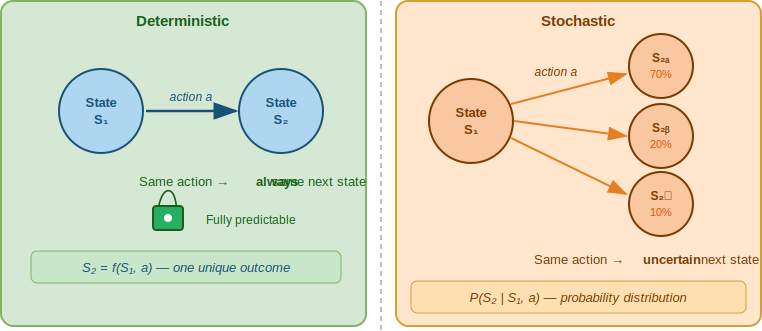
\includegraphics[width=.62\linewidth]{environment_determinism}
  			}
  			\only<3>{
				\smaller
				\begin{block}{Discrete Environment}
					\begin{itemize}
					\item \Emph{State space} and \Emph{action space} are finite or countably infinite
					\item Coordinates space is discrete and usually based on \Emph{integer values}
					\end{itemize}
				\end{block}
				\begin{block}{Continuous Environment}
					\begin{itemize}
					\item \Emph{State space} and \Emph{action space} are real-valued and potentially infinite-dimensional
					\item Coordinates space is continuous and usually based on \Emph{floating-point number values}
					\end{itemize}
				\end{block}
				\centering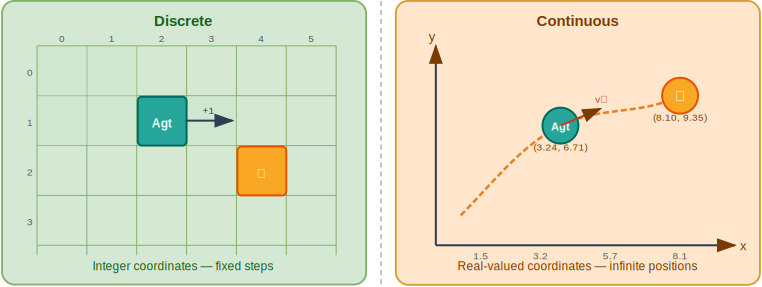
\includegraphics[width=.7\linewidth]{environment_dimensionality}
  			}
			\only<4>{
				\smaller
				\begin{block}{Dynamic Environment}
					\begin{itemize}
					\item Environment \Emph{may change over time}, independently of the agent's own actions
					\item Definition of endogenous dynamics engine
					\end{itemize}
				\end{block}
				\begin{block}{Static Environment}
					\begin{itemize}
					\item \Emph{Nothing changes} in the environment except as a direct result of the agent's own actions
					\end{itemize}
				\end{block}
				\centering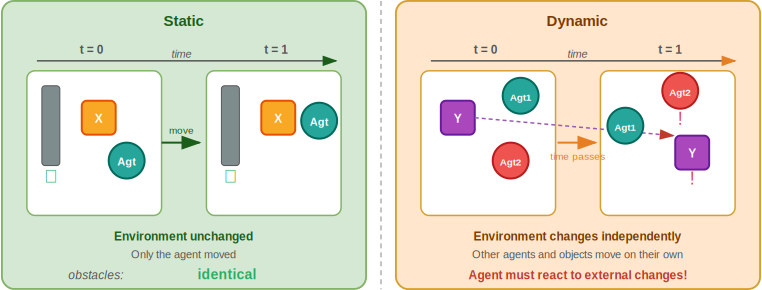
\includegraphics[width=.8\linewidth]{environment_dynamicity}
  			}
		\end{column}
	\end{columns}
\end{frame}

\sidecite{Weyns05}
\begin{frame}{Missions of the Environment}
	\begin{description}
	\item<1->[M1 - Sharing informations] Environment is a shared structure for agents, where each of them perceives and acts.
	\item<2->[M2 - Managing perception and observation] Agents can manage the access to environmental informations and guarantee the partialness and localness of perceptions.
	\item<3->[M3 - Managing agents actions and interactions] It is related to the management of agents' simultaneous and joint actions and to the preservation of the environmental integrity: influence-reaction model \cite{Ferber96,Michel04,GallandGaudDemangeKoukam2009_11}.
	\item<4->[M4 - Maintaining endogenous dynamics] The environment is an active entity; it can have its own processes, independently of the ones of the agents.
	\end{description}
\end{frame}

\sidecite{GallandGaudDemangeKoukam2009_11}
\figureslide{Agent Environment Model}{environment_model}

\sidecite{Michel.07,GallandGaudDemangeKoukam2009_11}
\figureslide{Body-Mind Distinction}{body_mind}

\end{graphicspathcontext}

\endinput

